%!TEX root=main.tex
\section{Experimental Evaluation}\label{sec:examples}
{\tiny
\begin{table}[!ht]
\begin{tabular}{l l}
\begin{minipage}[b]{0.45\linewidth}
    \centering
    \vspace{-0.5cm}
    \begin{tabular}{|l|l|l|l|l|l|l|l|}
    \hline
        Ex. & Sc. & L.Time & G.Time & It. & R.St. & T.St. & Res. \\ \hline
        \textsf{mut(2)} & 4 & 0.222 & 0.461 & 9 & $2^{2.58}$ & $2^{9.33}$ & F \\ \hline
        \textsf{mut(3)} & 4 & 0.204 & 0.877 & 27 & $2^3$ & $2^{13.50}$ & F \\ \hline
        \textsf{mut(4)} & 4 & 0.206 & 2.945 & 81 & $2^{3.32}$ & $ 2^{17.67}$ & F \\ \hline
        \textsf{mut(5)} & 4 & 0.208 & 11.05 & 243 & $ 2^{3.58}$ & $ 2^{21.84}$ & F \\ \hline
        \textsf{mut(6)} & 4 & 0.209 & 47.634 & 729 & $ 2^{3.80}$ & $ 2^{26.01}$ & F \\ \hline
        \textsf{mut(7)} & 4 & 0.21 & 220.863 & 2187 & $ 2^4$ & $ 2^{30.18}$ & F \\ \hline
        \textsf{phil(2)} & 14 & 0.904 & 1.226 & 5  & $2^4$ & $2^{14.33}$ & F \\ \hline
        \textsf{phil(3)} & 14 & 0.82 & 1.857 & 14 & $ 2^{5.95}$ & $2^{21.50}$ & F \\ \hline
        \textsf{phil(4)} & 14 & 0.801 & 5.987 & 41 & $2^8$ & $2^{28.67}$ & F \\ \hline
        \textsf{phil(5)} & 14 & 0.81 & 197.652 & 335 & $2^{9.39}$ & $2^{35.84}$ & F \\ \hline
        \textsf{phil(6)} & 14 & 0.808 & 973.321 & 365 & $2^{12}$ & $2^{43.01}$ & F \\ \hline
        \textsf{phil(7)} & 14 & 0.867 & TO & - & - & - & TO \\ \hline
        \textsf{bar(2)} & 16 & 0.768 & 1.535 & 11 & $2^{2.58}$ & $2^{14.58}$ & F \\ \hline
        \textsf{bar(3)} & 16 & 1.056 & 10.761 & 97 & $2^{5.90}$ & $2^{23.16}$ & F \\ \hline
        \textsf{bar(4)} & 16 & 2.978 & 62.111 & 85 & $2^{10.75}$ & $2^{32.16}$ & F \\ \hline
        \textsf{bar(5)} & 16 & 3.876 & TO & - & - & - & TO \\ \hline
        \textsf{pet(2)} & 12 & 0.414 & 0.511 & 2 & $2^2$ & $2^{8.16}$ & F \\ \hline
        \textsf{pet(3)} & 19 & TO & - & - & - & - & TO \\ \hline
        \textsf{pet(3)} & 20 & 238.777 & 239.337 & 5 & $2^{3.32}$ & $2^{16.22}$ & F \\ \hline
        \textsf{r(1)w(1)} & 6 & 0.28 & 0.446 & 7 & $2^{1.58}$ & $2^7$ & F \\ \hline
       \textsf{r(1)w(2)} & 6 & 0.323 & 0.865 & 25 & $2^2$ & $2^{10}$ & F \\ \hline
        \textsf{r(1)w(3)} & 6 & 0.361 & 2.112 & 79 & $2^{2.32}$ & $2^{13}$ & F \\ \hline
        \textsf{r(1)w(4)} & 6 & 0.389 & 6.211 & 241 & $2^{2.58}$ & $2^{16}$ & F \\ \hline
        \textsf{r(1)w(5)} & 6 & 0.441 & 19.625 & 723 & $2^{2.80}$ & $2^{19}$ & F \\ \hline
        \textsf{r(1)w(6)} & 6 & 0.459 & 67.666 & 2181 & $2^3$ & $2^{22}$ & F \\ \hline
        \textsf{r(2)w(1)} & 12 & 0.644 & 1.531 & 29 & $2^{2.32}$ & $2^{13.16}$ & F \\ \hline
        \textsf{r(2)w(2)} & 12 & 0.898 & 6.981 & 167 & $2^{2.58}$ & $ 2^{16.16}$ & F \\ \hline
        \textsf{r(2)w(3)} & 12 & 1.173 & 109.623 & 1377 & $2^{2.80}$ & $2^{19.16}$ & F \\ \hline
        \textsf{r(2)w(4)} & 11 & - & 0.8 & - & - & - & U \\ \hline
        \textsf{r(2)w(4)} & 12 & 1.565 & TO & - & - & - & TO\\ \hline
        \textsf{r(3)w(1)} & 24 & 37.757 & 38.192 & 4 & $ 2^{3.16}$ & ${2^{13}}$ & F \\ \hline
        \textsf{r(3)w(2)} & 24 & 74.951 & 76.572 & 13 & $ 2^{3.32}$ & $2^{16}$ & F \\ \hline
        \textsf{r(3)w(3)} & 24 & 109.623 & 113.523 & 40 & $2^{3.45}$ & $2^{19}$ & F \\ \hline
        \textsf{r(3)w(4)} & 24 & 147.42 & 159.073 & 121 & $2^{3.58}$ & $2^{22}$ & F \\ \hline
        \textsf{r(3)w(5)} & 24 & 184.087 & 235.318 & 362 & $2^{3.70}$ & ${2^{25}}$ & F \\ \hline
        \textsf{r(3)w(6)} & 24 & 220.121 & 382.628 & 1091 & $2^{3.80}$ & ${2^{28}}$ & F \\ \hline
\end{tabular}
\vspace{0.1cm}
\caption{Results for \textsf{mut}, \textsf{phil}, \textsf{bar}, \textsf{pet}, and \textsf{rw} examples.}\label{tab:results-common}
\end{minipage}
&
\begin{minipage}{0.70\textwidth}
\vspace{-17cm}
\centering
%MUTEX
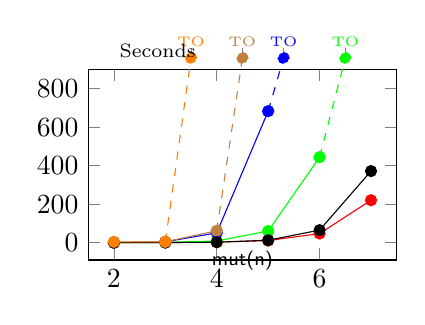
\begin{tikzpicture}
	\begin{axis}[name=Mutex,height=4cm,width=5.5cm,
		xlabel=\scriptsize{\textsf{mut(n)}},
		ylabel=\scriptsize{Seconds},
		x label style={at={(axis description cs:0.5,0.1)},anchor=north},
    	    y label style={at={(axis description cs:0.07,1.1)},anchor=west,rotate=-90},
    	%xmax=9,
		ymax=900,
		clip=false,
         %legend pos=north east
		]
    %exp2
	\addplot[color=red,mark=*] coordinates {
		(2, 0.461)
		(3, 0.877)
		(4, 2.945)
		(5, 11.05)
		(6, 47.634)
		(7, 220.863)
	};
	%exp4
	\addplot[color=green,mark=*] coordinates {
		(2, 0.483)
		(3, 1.602)
		(4, 9.032)
		(5, 60.845)
		(6, 444.691)
		%(6.5, 960) %time out
	};
	\addplot[color=green,mark=*,dashed] coordinates {		
		(6, 444.691)
		(6.5, 960) %time out
	}node[pin={[pin distance=-0.1cm]90:{\tiny{TO}}}]{};
	
	%exp8
	\addplot[color=blue,mark=*] coordinates {
		(2,0.983)
		(3,4.693)
		(4,51.233)
		(5,683.642)
		%(5.3,960) % time out
		%(7,1000)
		%(8,80.27)
		% (9,3600)
	};
	\addplot[color=blue,mark=*,dashed] coordinates {		
		(5,683.642)
		(5.3,960) % time out
		%(7,1000)
		%(8,80.27)
		% (9,3600)
	}node[pin={[pin distance=-0.1cm]90:{\tiny{TO}}}]{};
	
	%lineal10
	\addplot[color=brown,mark=*] coordinates {
		(2,0.608)
		(3,5.016)
		(4,62.034)
		%(4.5,960) % time out
		%(6,2.6)
		%(7,13.12)
		%(8,80.27)
		% (9,3600)
	};
	\addplot[color=brown,mark=*,dashed] coordinates {
		%(2,0.608)
		%(3,5.016)
		(4,62.034)
		(4.5,960) % time out
		%(6,2.6)
		%(7,13.12)
		%(8,80.27)
		% (9,3600)
	}node[pin={[pin distance=-0.1cm]90:{\tiny{TO}}}]{};
	%nocex
	\addplot[color=black,mark=*] coordinates {
		(2,0.348)
		(3,0.75)
		(4,2.679)
		(5,12.971)
		(6,65.403)
		(7,372.247)
		%(8,80.27)
		% (9,3600)
	};
	%psketch
	\addplot[color=orange,mark=*] coordinates {
		(2,4.62)
		(3,4.664)
		%(3.5,960)
		%(5,12.971)
		%(6,65.403)
		%(7,372.247)
		%(8,80.27)
		% (9,3600)
	};
	\addplot[color=orange,mark=*,dashed] coordinates {
		%(2,4.62)
		(3,4.664)
		(3.5,960)
		%(5,12.971)
		%(6,65.403)
		%(7,372.247)
		%(8,80.27)
		% (9,3600)
	}node[pin={[pin distance=-0.1cm]90:{\tiny{TO}}}]{};
	
	 %\addplot[color=black,mark=*] coordinates {
	% 	(9,3600)
	% } node[pin=180:{TO}]{};
	% \addplot[color=blue,dashed] coordinates {
	% 	(8,300)
	% 	(9,200)
	 %} node[pin=300:{TO}]{};
	%\addplot[color=green,mark=*,dashed] coordinates {
	%	(7,310)
		%(9, 107)
	%	} node[pin=180:{TO}]{};
	%\legend{exp2, exp4,exp8,lineal10,nocex}
	%\node[above right] at (rel axis cs:1, 1.1) {Time out:};
	%\node[above right] at (rel axis cs:0, 1) {\;\;\scriptsize{T.O:}};
	\end{axis}
\end{tikzpicture}
\label{fig:comparison}
% PHILOSOPHERS
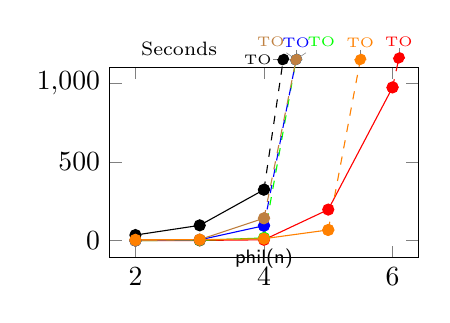
\begin{tikzpicture}
	\begin{axis}[name=Philosophers,height=4cm,width=5.5cm,
		xlabel=\scriptsize{\textsf{phil(n)}},
		ylabel=\scriptsize{Seconds},
		ymax=1100,
		clip=false,
		x label style={at={(axis description cs:0.5,0.1)},anchor=north},
    	y label style={at={(axis description cs:0.07,1.1)},anchor=west,rotate=-90},
		legend pos=north west]
    %exp2
	\addplot[color=red,mark=*] coordinates {
		(2,1.117)
		(3, 1.808)
		(4, 5.987)
		(5,197.652)
		(6,973.321)
		%(6.1,1160)
	};
	\addplot[color=red,mark=*,dashed] coordinates {
		(6,973.321)
		(6.1,1160)
	}node[pin={[pin distance=-0.1cm]90:{\tiny{TO}}}]{};
	%exp4
	\addplot[color=green,mark=*] coordinates {
		(2,1.253)
		(3, 2.765)
		(4, 17.661)
		%(4.5,1150)
		%(6,973.321)
		%(7,1000)
	};
	\addplot[color=green,mark=*,dashed] coordinates {
		(4, 17.661)
		(4.5,1150)
		%(6,973.321)
		%(7,1000)
	}node[pin={[pin distance=-0.1cm]60:{\tiny{TO}}}]{};
	
	%exp8
	\addplot[color=blue,mark=*] coordinates {
		(2,1.37)
		(3,5.552)
		(4,95.327)
		%(4.5,1150)
	     % (8,3600)
	};
	\addplot[color=blue,mark=*,dashed] coordinates {
		(4,95.327)
		(4.5,1150)
	     % (8,3600)
	}node[pin={[pin distance=-0.1cm]90:{\tiny{TO}}}]{};
	%lineal10
	\addplot[color=brown,mark=*] coordinates {
		(2,1.37)
		(3,7.264)
		(4,142.584)
		%(4.5,1150)
	     % (8,3600)
	};
	\addplot[color=brown,mark=*,dashed] coordinates {
		(4,142.584)
		(4.5,1150)
	     % (8,3600)
	}node[pin={[pin distance=-0.1cm]120:{\tiny{TO}}}]{};
	%nocex
	\addplot[color=black,mark=*] coordinates {
		(2,35.998)
		(3,97.636)
		(4,324)
		%(4.3,1150)
	     % (8,3600)
	};
	\addplot[color=black,mark=*,dashed] coordinates {
		(4,324)
		(4.3,1150)
	     % (8,3600)
	}node[pin={[pin distance=-0.1cm]180:{\tiny{TO}}}]{};
	%pskecth
	\addplot[color=orange,mark=*] coordinates {
		(2,5.916)
		(3,6.273)
		(4,12.845)%TO
		 (5,  68.5)
	     %(5.5,1150)
	};
	\addplot[color=orange,mark=*, dashed] coordinates {
		 (5,  68.5)
	     (5.5,1150)
	}node[pin={[pin distance=-0.1cm]90:{\tiny{TO}}}]{};
%\legend{exp2, PSketch}
     %\node[above right] at (rel axis cs:0, 1) {\;\;\scriptsize{T.O.:}};
	\end{axis}
\end{tikzpicture}
% BARRIER
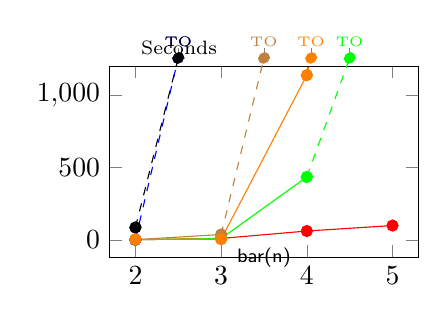
\begin{tikzpicture}
	\begin{axis}[name=SenseBarrier,height=4cm,width=5.5cm,
		xlabel=\scriptsize{\textsf{bar(n)}},
		ylabel=\scriptsize{Seconds},
		ymax=1200,
		clip=false,
		x label style={at={(axis description cs:0.5,0.1)},anchor=north},
    	y label style={at={(axis description cs:0.07,1.1)},anchor=west,rotate=-90},
		legend pos=north west]
    %exp2
	\addplot[color=red,mark=*] coordinates {
	    
		(2,1.535)
		(3, 10.761)
		(4, 62.111)
		(5,100)
		
	};
	%exp4
	\addplot[color=green,mark=*] coordinates {
	
		(2,1.672)
		(3, 10.569)
		(4, 436.365)
		%(4.5,1260) % TO
		%(6,973.321)
		%(7,1000)
	};
	\addplot[color=green,mark=*,dashed] coordinates {
		(4, 436.365)
		(4.5,1260) % TO
		%(6,973.321)
		%(7,1000)
	}node[pin={[pin distance=-0.1cm]90:{\tiny{TO}}}]{};
	
	%exp8
	\addplot[color=blue,mark=*] coordinates {
		(2,2.304)
	%	(2.5,1260)%TO
		%(4,95.327)
		%(5,1150)
	     % (8,3600)
	};
	\addplot[color=blue,mark=*,dashed] coordinates {
		(2,2.304)
		(2.5,1260)%TO
		%(4,95.327)
		%(5,1150)
	     % (8,3600)
	}node[pin={[pin distance=-0.1cm]90:{\tiny{TO}}}]{};
	%lineal10
	\addplot[color=brown,mark=*] coordinates {
	
		(2,2.362)
		(3,37.755)
		%(3.5,1260) % TO
		%(5,1150)
	     % (8,3600)
	};
	\addplot[color=brown,mark=*,dashed] coordinates {
	
		%(2,2.362)
		(3,37.755)
		(3.5,1260) % TO
		%(5,1150)
	     % (8,3600)
	}node[pin={[pin distance=-0.1cm]90:{\tiny{TO}}}]{};
	%nocex
	\addplot[color=black,mark=*] coordinates {
	   
		(2,86.916)
		%(2.5,1260)% TO
		%(4,324)
		%(4.3,1150)
	     % (8,3600)
	};
	\addplot[color=black,mark=*,dashed] coordinates {
	   
		(2,86.916)
		(2.5,1260)% TO
		%(4,324)
		%(4.3,1150)
	     % (8,3600)
	}node[pin={[pin distance=-0.1cm]90:{\tiny{TO}}}]{};
	%PSkecth
	\addplot[color=orange,mark=*] coordinates {
		(2,4.233)
		(3, 5.31)% TO
		(4,1140.9)
		%(4.05,1260)
	     % (8,3600)
	};
	\addplot[color=orange,mark=*,dashed] coordinates {
		(4,1140.9)
		(4.05,1260)
	     % (8,3600)
	}node[pin={[pin distance=-0.1cm]90:{\tiny{TO}}}]{};
%\legend{exp2, PSketch}
    %\node[above right] at (rel axis cs:0, 1) {\;\;\scriptsize{T.O.:}};
	\end{axis}
\end{tikzpicture}

% READERS & WRITERS
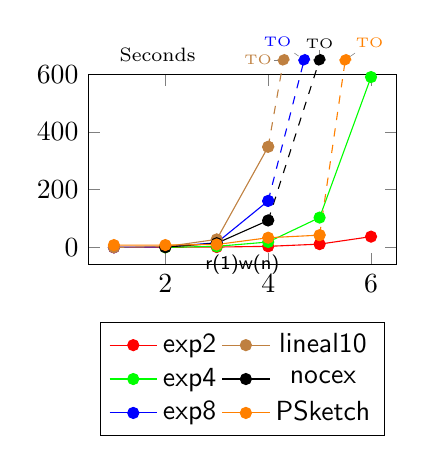
\begin{tikzpicture}
	\begin{axis}[name=Readers and Writers,height=4cm,width=5.5cm,
		xlabel=\scriptsize{\textsf{r(1)w(n)}},
		ylabel=\scriptsize{Seconds},
		x label style={at={(axis description cs:0.5,0.1)},anchor=north},
    	y label style={at={(axis description cs:0.07,1.1)},anchor=west,rotate=-90},
    	ymax=600,
		clip=false,
		legend style={at={(0.5,-0.3)},anchor=north,legend  columns =3, transpose legend}]
    % exp2
     \addlegendimage{red, line legend, mark=*} % or mark=none?
    \addlegendentry{\textsf{exp2}}
    \addlegendimage{green, line legend, , mark=*} % or mark=none?
    \addlegendentry{\textsf{exp4}}
    \addlegendimage{blue, line legend, , mark=*} % or mark=none?
    \addlegendentry{\textsf{exp8}}
    \addlegendimage{brown, line legend, , mark=*} % or mark=none?
    \addlegendentry{\textsf{lineal10}}
    \addlegendimage{black,,line legend,  mark=*} % or mark=none?
    \addlegendentry{\textsf{nocex}}
    \addlegendimage{orange,,line legend,  mark=*} % or mark=none?
    \addlegendentry{\textsf{PSketch}}
	\addplot[color=red,mark=*] coordinates {
		(1,0.492)
		(2,0.813)
		(3,1.603)
		(4,4.069)
		(5,11.705)
		(6,37.703)
	};
	% exp4
	\addplot[color=green,mark=*] coordinates {
		%(1,0.439)
		(2,0.442)
		(3,4.055)
		(4,19.064)
		(5,103.635)
		(6,590.277)
	};
	% exp8
	\addplot[color=blue,mark=*] coordinates {
		(1,0.625)
		(2,2.247)
		(3,16.51)
		(4,161.499)
		%(5,600) %TO
	};
	\addplot[color=blue,mark=*,dashed] coordinates {
		(4,161.499)
		(4.7,650) %TO
	}node[pin={[pin distance=-0.1cm]130:{\tiny{TO}}}]{};
	%lineal10
	\addplot[color=brown,mark=*] coordinates {
		(1,0.654)
		(2,2.892)
		(3,28.208)
		(4,348.931)
		%(4.3,660) %TO
	};
	\addplot[color=brown,mark=*,dashed] coordinates {
		(4,348.931)
		(4.3,650) %TO
	}node[pin={[pin distance=-0.1cm]180:{\tiny{TO}}}]{};
	\addplot[color=black,mark=*] coordinates {
		%(1,0.511)
		(2,1.344)
		(3,14.807)
		(4,93.844)
		%(5,600) %TO
	};
	\addplot[color=black,mark=*,dashed] coordinates {
		%(1,0.511)
		(4,93.844)
		(5,650) %TO
	}node[pin={[pin distance=-0.1cm]90:{\tiny{TO}}}]{};
	
	%PSketch
	\addplot[color=orange,mark=*] coordinates {
		(1,8.465)
		(2,8.483)
		(3,10.463)
		(4,33.898)
		(5,42.824)
		%(6,600)%TO
	};
	\addplot[color=orange,mark=*,dashed] coordinates {
		(5,42.824)
		(5.5,650)%TO
	}node[pin={[pin distance=-0.1cm]70:{\tiny{TO}}}]{};
   %\legend{exp2,exp4,exp8,lineal10,nocex,psketch}
    %\node[above right] at (rel axis cs:0, 1) {\;\;\scriptsize{T.O.:}};
	\end{axis}
\end{tikzpicture}
\vspace{0.4cm}
\captionof{figure}{Comparison between \\ \textsf{exp2}, \textsf{exp4}, \textsf{exp8},  \textsf{lineal10},  \textsf{nocex}, \\ and {\PSketch}.}
\label{fig:examples-plot}
\end{minipage}
\end{tabular}
\vspace{-0.5cm}
\end{table}
}
%{\scriptsize
%\begin{table}[!ht]
%\begin{tabular}{l l}
%\begin{minipage}{0.67\linewidth}
%    \centering
%    \begin{tabular}{|l|l|l|l|l|l|l|l|}
%    \hline
%        Ex. & Sc. & L.Time & G.Time & It. & R.St. & T.St. & Res. \\ \hline
%        Arb2 & 12 & 0.814 &  1.322 & 7 & $2^{2.32}$  & $2^{12}$ & F \\ \hline
%        Arb3 & 12 & 0.728 & 2.11 & 16 & $2^4$ & $2^18$ & F \\ \hline
%        Arb4 & 12 & 0.854 & 4.303 & 16 & $2^{5.24}$ & $2^{24}$ & F \\ \hline
%        Arb5 & 12 & 0.976 & 12.54 & 16 & $2^{6.35}$ & $2^{30}$ & F \\ \hline
%        Arb6 & 12 & 1.134 & 52.344 & 16 & $2^{7.40}$ & $2^{36}$ & F \\ \hline
%        FArb2 & 12 & 0.552 & 1.164 & 8 & $2^{2.58}$ & $2^{12}$ & F \\ \hline
%        FArb3 & 12 & 0.75 & 2.97 & 20 & $2^{3.45}$ & $2^{18}$ & F \\ \hline
%        FArb4 & 12 & 0.935 & 15.602 & 56 & $2^{4.39}$ & $2^{24}$ & F \\ \hline
%        FArb5 & 12 & 1.232 & 85.933 & 164 & $2^{5.35}$ & $2^{30}$ & F \\ \hline
%        FArb6 & 12 & 2.034 & 1004.49 & 857 & - & - & NF\\ \hline
%        FArb2 & 12 & 0.662 & 1.166 & 8 & $2^{2.80}$ & $2^{12}$ & F\\ \hline
%        PArb3 & 12 & 0.714 & 2.277 & 20 & $2^{3.45}$ & $2^{18}$ & F \\ \hline
%        PArb4 & 12 & 0.886 & 8.593 & 56 & $2^{4.39}$ & $2^{24}$ & F\\ \hline
%        PArb5 & 12 & 1.092 & 54.25 & 164 & $2^{5.35}$ & $2^{30}$ & F \\ \hline
%        PArb6 & 12 &1.324 & 700.731 & 488 & $2^{6.33}$ & $2^{36}$ & F \\ \hline
%    \end{tabular}
%\caption{Results for the Arbiter examples.}\label{tab:results-arbiter}
%\end{minipage}
%\begin{minipage}{0.50\linewidth}
%\centering
%\begin{tikzpicture}
%	\begin{axis}[name=Arbiter,height=4cm,width=5.5cm,
%		xlabel=\scriptsize{Arbiter(n)},
%		ylabel=\scriptsize{Seconds},
%		x label style={at={(axis description cs:0.5,0.1)},anchor=north},
%    	y label style={at={(axis description cs:0.07,1.1)},anchor=west,rotate=-90},
%    	ymax=75,
%		clip=false,
%		legend pos=north west]
%    % exp2
%	\addplot[color=red,mark=*] coordinates {
%		(2,0.768)
%		(3,1.563)
%		(4,2.175)
%		(5,3.768)
%		(6,9.172)
%		%(6,37.703)
%	};
%	% exp4
%	\addplot[color=green,mark=*] coordinates {
%		(2,0.78)
%		(3,1.687)
%		(4,3.085)
%		(5,6.985)
%		(6,19.659)
%	};
%	% exp8
%	\addplot[color=blue,mark=*] coordinates {
%		(2,0.67)
%		(3,2.132)
%		(4,4)
%		(5,10.624)
%		(6, 35.653) 
%	};
%	%lineal10
%	\addplot[color=brown,mark=*] coordinates {
%		(2,0.972)
%		(3,3.359)
%		(4,7.829)
%		(5,16.491)
%		(6,54.652)
%	};
%	%Party
%	\addplot[color=pink,mark=*] coordinates {
%		(2,0.63)
%		(3,1.18)
%		(4,2.82)
%		(5,6.12)
%		(6,12.43)
%	};
%	%nocex
%	%\addplot[color=black,mark=x] coordinates {
%	%	(1,0.511)
%	%	(2,1.344)
%	%	(3,14.807)
%	%	(4,93.844)
%	%	(5,600) %TO
%	%};
%	
%%\legend{exp2,exp4,exp8,lineal10,nocex}
%    \node[above right] at (rel axis cs:0, 1) {\;\;\scriptsize{Time out:}};
%	\end{axis}
%\end{tikzpicture}
%%Full Arbiter
%\begin{tikzpicture}
%	\begin{axis}[name=FullArbiter,height=4cm,width=5.5cm,
%		xlabel=\scriptsize{FullArbiter(n)},
%		ylabel=\scriptsize{Seconds},
%		x label style={at={(axis description cs:0.5,0.1)},anchor=north},
%    	y label style={at={(axis description cs:0.07,1.1)},anchor=west,rotate=-90},
%    	ymax=1200,
%		clip=false,
%		legend pos=north west]
%    % exp2
%	\addplot[color=red,mark=*] coordinates {
%		(2,1.164)
%		(3,2.97)
%		(4,15.609)
%		(5,85.933)
%		(6,1004.49)
%		%(6,37.703)
%	};
%	% exp4
%	\addplot[color=green,mark=*] coordinates {
%		(2,0.8)
%		(3,1.466)
%		(4,3.457)
%		(5,10.8)
%		(6,66.433)
%	};
%	% exp8
%	\addplot[color=blue,mark=*] coordinates {
%		(2,0.83)
%		(3,1.507)
%		(4,3.562)
%		(5,12.345)
%		(6, 69.144) %TO
%	};
%	%lineal10
%	\addplot[color=brown,mark=*] coordinates {
%		(2,2.024)
%		(3,19.822)
%		(4,298.955)
%		(5,1200)%TO
%	};
%	\addplot[color=pink,mark=*] coordinates {
%		(2,0.68)
%		(3,1.43)
%		(4,4.078)
%		(5,8.85)
%		(6,32.73)
%	};
%	%nocex
%	%\addplot[color=black,mark=x] coordinates {
%	%	(1,0.511)
%	%	(2,1.344)
%	%	(3,14.807)
%	%	(4,93.844)
%	%	(5,600) %TO
%	%};
%%\legend{exp2,exp4,exp8,lineal10,nocex}
%    \node[above right] at (rel axis cs:0, 1) {\;\;\scriptsize{Time out:}};
%	\end{axis}
%\end{tikzpicture}
%%PNUELIARBITER
%\begin{tikzpicture}
%	\begin{axis}[name=PnueliArbiter,height=4cm,width=5.5cm,
%		xlabel=\scriptsize{PnueliArbiter(n)},
%		ylabel=\scriptsize{Seconds},
%		x label style={at={(axis description cs:0.5,0.1)},anchor=north},
%    	y label style={at={(axis description cs:0.07,1.1)},anchor=west,rotate=-90},
%    	ymax=1400,
%		clip=false,
%		legend style={at={(0.2,-0.5)},anchor=north}]
%    % exp2
%	\addplot[color=red,mark=*] coordinates {
%		(2,1.168)
%		(3,2.277)
%		(4,8.593)
%		(5,54.25)
%		(6,1362.85) % TO
%		%(6,37.703)
%	};
%	% exp4
%	\addplot[color=green,mark=*] coordinates {
%		(2,0.676)
%		(3,1.146)
%		(4,2.355)
%		(5,11.6)
%		(6,66.433) 
%	};
%	% exp8
%	\addplot[color=blue,mark=*] coordinates {
%		(2,0.707)
%		(3,1.242)
%		(4,2.433)
%		(5,12.173)
%		(6, 65.155) %TO
%	};
%	%lineal10
%	\addplot[color=brown,mark=*] coordinates {
%		(2,0.69)
%		(3,1.162)
%		(4,2.408)
%		(5,11.836)
%		(6,59.299)
%	};
%	%nocex
%	%\addplot[color=black,mark=x] coordinates {
%	%	(1,0.511)
%	%	(2,1.344)
%	%	(3,14.807)
%	%	(4,93.844)
%	%	(5,600) %TO
%	%};
%	%party
%	\addplot[color=pink,mark=*] coordinates {
%		(2,0.69)
%		(3,1.162)
%		(4,2.408)
%		(5,11.836)
%		(6,1400)
%	};
%\legend{exp2,exp4,exp8,lineal10,nocex}
%    \node[above right] at (rel axis cs:0, 1) {\;\;\scriptsize{Time out:}};
%	\end{axis}
%\end{tikzpicture}
%\end{minipage}
%\end{tabular}
%\end{table}
%}

%\begin{figure}[hbt!]
%\begin{tabular}{l l}
%\begin{minipage}{0.48\linewidth}
%\centering
%%MUTEX
%\begin{tikzpicture}
%	\begin{axis}[name=Mutex,height=4cm,width=5.5cm,
%		xlabel=\scriptsize{Mutex(n)},
%		ylabel=\scriptsize{Seconds},
%		x label style={at={(axis description cs:0.5,0.1)},anchor=north},
%    	    y label style={at={(axis description cs:0.07,1.1)},anchor=west,rotate=-90},
%    	%xmax=9,
%		ymax=900,
%		clip=false,
%         %legend pos=north east
%		]
%    %exp2
%	\addplot[color=red,mark=*] coordinates {
%		(2, 0.461)
%		(3, 0.877)
%		(4, 2.945)
%		(5, 11.05)
%		(6, 47.634)
%		(7, 220.863)
%	};
%	%exp4
%	\addplot[color=green,mark=*] coordinates {
%		(2, 0.483)
%		(3, 1.602)
%		(4, 9.032)
%		(5, 60.845)
%		(6, 444.691)
%		(7, 900) %time out
%	};
%	%exp8
%	\addplot[color=blue,mark=*] coordinates {
%		(2,0.983)
%		(3,4.693)
%		(4,51.233)
%		(5,683.642)
%		(5.3,900) % time out
%		%(7,1000)
%		%(8,80.27)
%		% (9,3600)
%	};
%	%lineal10
%	\addplot[color=brown,mark=*] coordinates {
%		(2,0.608)
%		(3,5.016)
%		(4,62.034)
%		(5,900) % time out
%		%(6,2.6)
%		%(7,13.12)
%		%(8,80.27)
%		% (9,3600)
%	};
%	%nocex
%	\addplot[color=black,mark=*] coordinates {
%		(2,0.348)
%		(3,0.75)
%		(4,2.679)
%		(5,12.971)
%		(6,65.403)
%		(7,372.247)
%		%(8,80.27)
%		% (9,3600)
%	};
%	 %\addplot[color=black,mark=*] coordinates {
%	% 	(9,3600)
%	% } node[pin=180:{TO}]{};
%	% \addplot[color=blue,dashed] coordinates {
%	% 	(8,300)
%	% 	(9,200)
%	 %} node[pin=300:{TO}]{};
%	%\addplot[color=green,mark=*,dashed] coordinates {
%	%	(7,310)
%		%(9, 107)
%	%	} node[pin=180:{TO}]{};
%	%\legend{exp2, exp4,exp8,lineal10,nocex}
%	%\node[above right] at (rel axis cs:1, 1.1) {Time out:};
%	\node[above right] at (rel axis cs:0, 1) {\;\;\scriptsize{Time out:}};
%	\end{axis}
%\end{tikzpicture}
%\label{fig:comparison}
%% PHILOSOPHERS
%\begin{tikzpicture}
%	\begin{axis}[name=Philosophers,height=4cm,width=5.5cm,
%		xlabel=\scriptsize{Phils(n)},
%		ylabel=\scriptsize{Seconds},
%		ymax=1100,
%		clip=false,
%		x label style={at={(axis description cs:0.5,0.1)},anchor=north},
%    	y label style={at={(axis description cs:0.07,1.1)},anchor=west,rotate=-90},
%		legend pos=north west]
%    %exp2
%	\addplot[color=red,mark=*] coordinates {
%		(2,1.117)
%		(3, 1.808)
%		(4, 5.987)
%		(5,197.652)
%		(6,973.321)
%		(6.1,1100)
%	};
%	%exp4
%	\addplot[color=green,mark=*] coordinates {
%		(2,1.253)
%		(3, 2.765)
%		(4, 17.661)
%		(5,1100)
%		%(6,973.321)
%		%(7,1000)
%	};
%	%exp8
%	\addplot[color=blue,mark=*] coordinates {
%		(2,1.37)
%		(3,5.552)
%		(4,95.327)
%		(5,1100)
%	     % (8,3600)
%	};
%	%lineal10
%	\addplot[color=brown,mark=*] coordinates {
%		(2,1.37)
%		(3,7.264)
%		(4,142.584)
%		(5,1100)
%	     % (8,3600)
%	};
%	%nocex
%	\addplot[color=black,mark=*] coordinates {
%		(2,35.998)
%		(3,97.636)
%		(4,324)
%		(4.3,1100)
%	     % (8,3600)
%	};
%%\legend{exp2, PSketch}
%     \node[above right] at (rel axis cs:0, 1) {\;\;\scriptsize{Time out:}};
%	\end{axis}
%\end{tikzpicture}
%% BARRIER
%\begin{tikzpicture}
%	\begin{axis}[name=SenseBarrier,height=4cm,width=5.5cm,
%		xlabel=\scriptsize{SenseBarrier(n)},
%		ylabel=\scriptsize{Seconds},
%		ymax=500,
%		clip=false,
%		x label style={at={(axis description cs:0.5,0.1)},anchor=north},
%    	y label style={at={(axis description cs:0.07,1.1)},anchor=west,rotate=-90},
%		legend pos=north west]
%    %exp2
%	\addplot[color=red,mark=*] coordinates {
%	    
%		(2,1.535)
%		(3, 10.761)
%		(4, 62.111)
%		(5,100)
%		
%	};
%	%exp4
%	\addplot[color=green,mark=*] coordinates {
%	
%		(2,1.672)
%		(3, 10.569)
%		(4, 436.365)
%		(4.1,500) % TO
%		%(6,973.321)
%		%(7,1000)
%	};
%	%exp8
%	\addplot[color=blue,mark=*] coordinates {
%	
%		(2,2.304)
%		(3,500)%TO
%		%(4,95.327)
%		%(5,1150)
%	     % (8,3600)
%	};
%	%lineal10
%	\addplot[color=brown,mark=*] coordinates {
%	
%		(2,2.362)
%		(3,37.755)
%		(4,500) % TO
%		%(5,1150)
%	     % (8,3600)
%	};
%	%nocex
%	\addplot[color=black,mark=*] coordinates {
%	   
%		(2,86.916)
%		(2.5,500)% TO
%		%(4,324)
%		%(4.3,1150)
%	     % (8,3600)
%	};
%%\legend{exp2, PSketch}
%    \node[above right] at (rel axis cs:0, 1) {\;\;\scriptsize{Time out:}};
%	\end{axis}
%\end{tikzpicture}
%
%% READERS & WRITERS
%\begin{tikzpicture}
%	\begin{axis}[name=Readers and Writers,height=4cm,width=5.5cm,
%		xlabel=\scriptsize{RW(1,n)},
%		ylabel=\scriptsize{Seconds},
%		x label style={at={(axis description cs:0.5,0.1)},anchor=north},
%    	y label style={at={(axis description cs:0.07,1.1)},anchor=west,rotate=-90},
%    	ymax=600,
%		clip=false,
%		legend pos=north west]
%    % exp2
%	\addplot[color=red,mark=*] coordinates {
%		(1,0.492)
%		(2,0.813)
%		(3,1.603)
%		(4,4.069)
%		(5,11.705)
%		(6,37.703)
%	};
%	% exp4
%	\addplot[color=green,mark=*] coordinates {
%		(1,0.439)
%		(2,0.442)
%		(3,4.055)
%		(4,19.064)
%		(5,103.635)
%		(6,590.277)
%	};
%	% exp8
%	\addplot[color=blue,mark=*] coordinates {
%		(1,0.625)
%		(2,2.247)
%		(3,16.51)
%		(4,161.499)
%		(5,600) %TO
%	};
%	%lineal10
%	\addplot[color=brown,mark=*] coordinates {
%		(1,0.654)
%		(2,2.892)
%		(3,28.208)
%		(4,348.931)
%		(4.3,600) %TO
%	};
%	\addplot[color=black,mark=*] coordinates {
%		(1,0.511)
%		(2,1.344)
%		(3,14.807)
%		(4,93.844)
%		(5,600) %TO
%	};
%
%%\legend{exp2,exp4,exp8,lineal10,nocex}
%    \node[above right] at (rel axis cs:0, 1) {\;\;\scriptsize{Time out:}};
%	\end{axis}
%\end{tikzpicture}
%\end{minipage}
%%\captionof{figure}{Comparison for exp2, exp4, exp8, lineal10, and nocex.}
%&
%%%% ARBITER EXAMPLES
%%Arbiter
%\begin{minipage}{0.48\linewidth}
%\centering
%\begin{tikzpicture}
%	\begin{axis}[name=Arbiter,height=4cm,width=5.5cm,
%		xlabel=\scriptsize{Arbiter(n)},
%		ylabel=\scriptsize{Seconds},
%		x label style={at={(axis description cs:0.5,0.1)},anchor=north},
%    	y label style={at={(axis description cs:0.07,1.1)},anchor=west,rotate=-90},
%    	ymax=75,
%		clip=false,
%		legend pos=north west]
%    % exp2
%	\addplot[color=red,mark=*] coordinates {
%		(2,0.768)
%		(3,1.563)
%		(4,2.175)
%		(5,3.768)
%		(6,9.172)
%		%(6,37.703)
%	};
%	% exp4
%	\addplot[color=green,mark=*] coordinates {
%		(2,0.78)
%		(3,1.687)
%		(4,3.085)
%		(5,6.985)
%		(6,19.659)
%	};
%	% exp8
%	\addplot[color=blue,mark=*] coordinates {
%		(2,0.67)
%		(3,2.132)
%		(4,4)
%		(5,10.624)
%		(6, 35.653) 
%	};
%	%lineal10
%	\addplot[color=brown,mark=*] coordinates {
%		(2,0.972)
%		(3,3.359)
%		(4,7.829)
%		(5,16.491)
%		(6,54.652)
%	};
%	%Party
%	\addplot[color=pink,mark=*] coordinates {
%		(2,0.63)
%		(3,1.18)
%		(4,2.82)
%		(5,6.12)
%		(6,12.43)
%	};
%	%nocex
%	%\addplot[color=black,mark=x] coordinates {
%	%	(1,0.511)
%	%	(2,1.344)
%	%	(3,14.807)
%	%	(4,93.844)
%	%	(5,600) %TO
%	%};
%	
%%\legend{exp2,exp4,exp8,lineal10,nocex}
%    \node[above right] at (rel axis cs:0, 1) {\;\;\scriptsize{Time out:}};
%	\end{axis}
%\end{tikzpicture}
%%Full Arbiter
%\begin{tikzpicture}
%	\begin{axis}[name=FullArbiter,height=4cm,width=5.5cm,
%		xlabel=\scriptsize{FullArbiter(n)},
%		ylabel=\scriptsize{Seconds},
%		x label style={at={(axis description cs:0.5,0.1)},anchor=north},
%    	y label style={at={(axis description cs:0.07,1.1)},anchor=west,rotate=-90},
%    	ymax=1200,
%		clip=false,
%		legend pos=north west]
%    % exp2
%	\addplot[color=red,mark=*] coordinates {
%		(2,1.164)
%		(3,2.97)
%		(4,15.609)
%		(5,85.933)
%		(6,1004.49)
%		%(6,37.703)
%	};
%	% exp4
%	\addplot[color=green,mark=*] coordinates {
%		(2,0.8)
%		(3,1.466)
%		(4,3.457)
%		(5,10.8)
%		(6,66.433)
%	};
%	% exp8
%	\addplot[color=blue,mark=*] coordinates {
%		(2,0.83)
%		(3,1.507)
%		(4,3.562)
%		(5,12.345)
%		(6, 69.144) %TO
%	};
%	%lineal10
%	\addplot[color=brown,mark=*] coordinates {
%		(2,2.024)
%		(3,19.822)
%		(4,298.955)
%		(5,1200)%TO
%	};
%	\addplot[color=pink,mark=*] coordinates {
%		(2,0.68)
%		(3,1.43)
%		(4,4.078)
%		(5,8.85)
%		(6,32.73)
%	};
%	%nocex
%	%\addplot[color=black,mark=x] coordinates {
%	%	(1,0.511)
%	%	(2,1.344)
%	%	(3,14.807)
%	%	(4,93.844)
%	%	(5,600) %TO
%	%};
%%\legend{exp2,exp4,exp8,lineal10,nocex}
%    \node[above right] at (rel axis cs:0, 1) {\;\;\scriptsize{Time out:}};
%	\end{axis}
%\end{tikzpicture}
%%PNUELIARBITER
%\begin{tikzpicture}
%	\begin{axis}[name=PnueliArbiter,height=4cm,width=5.5cm,
%		xlabel=\scriptsize{PnueliArbiter(n)},
%		ylabel=\scriptsize{Seconds},
%		x label style={at={(axis description cs:0.5,0.1)},anchor=north},
%    	y label style={at={(axis description cs:0.07,1.1)},anchor=west,rotate=-90},
%    	ymax=1400,
%		clip=false,
%		legend style={at={(0.2,-0.5)},anchor=north}]
%    % exp2
%	\addplot[color=red,mark=*] coordinates {
%		(2,1.168)
%		(3,2.277)
%		(4,8.593)
%		(5,54.25)
%		(6,1362.85) % TO
%		%(6,37.703)
%	};
%	% exp4
%	\addplot[color=green,mark=*] coordinates {
%		(2,0.676)
%		(3,1.146)
%		(4,2.355)
%		(5,11.6)
%		(6,66.433) 
%	};
%	% exp8
%	\addplot[color=blue,mark=*] coordinates {
%		(2,0.707)
%		(3,1.242)
%		(4,2.433)
%		(5,12.173)
%		(6, 65.155) %TO
%	};
%	%lineal10
%	\addplot[color=brown,mark=*] coordinates {
%		(2,0.69)
%		(3,1.162)
%		(4,2.408)
%		(5,11.836)
%		(6,59.299)
%	};
%	%nocex
%	%\addplot[color=black,mark=x] coordinates {
%	%	(1,0.511)
%	%	(2,1.344)
%	%	(3,14.807)
%	%	(4,93.844)
%	%	(5,600) %TO
%	%};
%	%party
%	\addplot[color=pink,mark=*] coordinates {
%		(2,0.69)
%		(3,1.162)
%		(4,2.408)
%		(5,11.836)
%		(6,1400)
%	};
%\legend{exp2,exp4,exp8,lineal10,nocex}
%    \node[above right] at (rel axis cs:0, 1) {\;\;\scriptsize{Time out:}};
%	\end{axis}
%\end{tikzpicture}
%\vspace{1.3cm}
%
%%\captionof{figure}{Comparison with Party Tool.}
%\label{fig:comparison}
%\end{minipage}
%\end{tabular}
%\end{figure}
We evaluate our approach around the following research questions: 
\begin{description}
\item[RQ1] \emph{How effective/efficient is our synthesis approach?}
\item[RQ2] \emph{How good is the counterexample-guided search for speeding up the synthesis method?}
\item[RQ3] \emph{How do the selected bounds affect the synthesis method?}
\item[RQ4] \emph{How does our approach compare with related approaches?}
\end{description}
To answer these questions,  we implemented Alg.~\ref{alg:improved_alg} in a prototype tool, it uses the \textsf{Alloy Analyzer}~\cite{AlloyBook} for obtaining instances of specifications, and {\NuSMV}~\cite{Cimatti+2002} for model checking the candidates.  We evaluate our approach on eight  examples of distributed algorithms: the dining philosophers (\textsf{phil})~\cite{Dijkstra71} (our running example), Mutex (\textsf{mut})~\cite{Fokkink13},  Readers and Writers (\textsf{rw})~\cite{Fokkink13}, the generalized version of Peterson's algorithm (\textsf{pet})~\cite{Fokkink13},   and the combined-tree Barrier protocol (\textsf{bar})~\cite{Fokkink13}.  Furthermore,  we  also encoded the arbiter examples presented in \cite{Party,Piterman+2006}: a simple arbiter (\textsf{arb}), a full arbiter (\textsf{farb}), and the Pnueli arbiter (\textsf{parb}). These case studies assume a distributed token ring architecture,  which we modeled using the Alloy language.  

%\cite{PhilStone}. The tool takes as input a  specification and returns, when possible, an LTS satisfying the specification, described in the \NuSMV  language.
Tables~\ref{tab:results-common} and~\ref{tab:results-arbiter}  summarize the experimental results. The experiments were conducted on an Apple M2 processor with 16GB of memory.   In these examples, we used the sequence of bounds $2,4,8,16,\dots$, named \textsf{exp2} from now on.
For each case study, we report the 
bound over the size of the processes (Sc), the maximum time needed to generate local process instances (L.Time), the total time required for synthesizing the system (T.Time), the number of times that the model checker was invoked (Its) by the synthesizer, and the final result of our synthesis algorithm:  `F' (if an implementation was found),  `N'  (if no implementation was found),  `TO'  if the example timed out, or `U'  (if the specification was found unsatisfiable by the Alloy tool).  We also report the number of reachable states (R.St.), and the total states (T.St.) of the obtained implementations, expressed as power of $2$.  For space reasons, we only include a few configurations found unsatisfiable by the solver; similar numbers can be obtained for the rest of the cases if the specifications are processed with smaller scopes. We also indicate the number of processes considered in each experiment.  For instance,  \textsf{phil(6)} indicates that we considered \textsf{6} concurrent processes (i.e., philosophers) in the dining philosophers example. In the case of Readers and Writers, 
\textsf{r(n)w(m)} means that \textsf{n} readers and \textsf{m} writers were considered.  We  have  set out a time out of 30 minutes.
\begin{wraptable}[19]{r}{.60\textwidth}
\vspace{-0.5cm}
\begin{tabular}{|l|l|l|l|l|l|l|l|}
    \hline
        Ex. & Sc. & L.Time & G.Time & It. & R.St. & T.St. & Res. \\ \hline
        \textsf{arb(2)} & 12 & 0.814 &  1.322 & 7 & $2^{2.32}$  & $2^{12}$ & F \\ \hline
        \textsf{arb(3)} & 12 & 0.728 & 2.11 & 16 & $2^4$ & $2^{18}$ & F \\ \hline
        \textsf{arb(4)} & 12 & 0.854 & 4.303 & 16 & $2^{5.24}$ & $2^{24}$ & F \\ \hline
        \textsf{arb(5)} & 12 & 0.976 & 12.54 & 16 & $2^{6.35}$ & $2^{30}$ & F \\ \hline
        \textsf{arb(6)} & 12 & 1.134 & 52.344 & 16 & $2^{7.40}$ & $2^{36}$ & F \\ \hline
        \textsf{farb(2)} & 12 & 0.552 & 1.164 & 8 & $2^{2.58}$ & $2^{12}$ & F \\ \hline
        \textsf{farb(3)} & 12 & 0.75 & 2.97 & 20 & $2^{3.45}$ & $2^{18}$ & F \\ \hline
        \textsf{farb(4)} & 12 & 0.935 & 15.602 & 56 & $2^{4.39}$ & $2^{24}$ & F \\ \hline
        \textsf{farb(5)} & 12 & 1.232 & 85.933 & 164 & $2^{5.35}$ & $2^{30}$ & F \\ \hline
        \textsf{farb(6)} & 12 & 2.034 & 672.539 & 488 & $2^{6.33}$ & $2^{36}$ & F\\ \hline
        \textsf{parb(2)} & 12 & 0.662 & 1.166 & 8 & $2^{2.80}$ & $2^{12}$ & F\\ \hline
        \textsf{parb(3)} & 12 & 0.714 & 2.277 & 20 & $2^{3.45}$ & $2^{18}$ & F \\ \hline
        \textsf{parb(4)} & 12 & 0.886 & 8.593 & 56 & $2^{4.39}$ & $2^{24}$ & F\\ \hline
        \textsf{parb(5)} & 12 & 1.092 & 54.25 & 164 & $2^{5.35}$ & $2^{30}$ & F \\ \hline
        \textsf{parb(6)} & 12 &1.324 & 700.731 & 488 & $2^{6.33}$ & $2^{36}$ & F \\ \hline
\end{tabular}
\caption{Results for the arbiter examples.}\label{tab:results-arbiter}
\end{wraptable}
%
Table \ref{tab:results-common} shows that the technique scales reasonably well for those case studies in which each process uses only a reduced number of locks and shared variables (e.g., dining philosophers, mutex and reader-writers). For the cases where the number of shared variables accessed by the processes is bigger (e.g., Peterson for $n$ processes), the technique does not scale that well. Intuitively, more shared variables imply more actions performed by the environment, which increases the size of the formula fed to the SAT solver.  We plan to investigate how to equip specifications with assumptions on the environment's behavior, to restrict the possible values of shared variables; this may simplify the SAT problem when searching for local implementations.  It is worth noting, that even though the algorithm is incomplete, we have not 
observed any ``not found'' outputs in our benchmarks. This could be due to  the set timeouts.  We leave an in-depth investigation of this as further work.

 To answer \textbf{RQ3}   we compare the results obtained with several configurations of bounds for the exploration phase, namely: \textsf{exp4} ($4,16,64,\dots$),  \textsf{exp8} ($8,64,512,\dots$),  \textsf{lineal10} ($10,20,30,\dots$), and for \textbf{RQ2} we also considered Alg.~\ref{alg:the_alg},  which does not take into account counterexamples (\textsf{nocex}).  The obtained results are depicted in Figs.\ref{fig:examples-plot} and \ref{fig:arbiter-plots}.  Note that time outs are remarked using dashed lines going out of the $y$-axis.
 In general, \textsf{exp2} behaves better than the other options,  thus it seems better to collect a few counterexamples first, and use them to improve the search.  A possible drawback of this setting is that a wrong choice of the first counterexamples may have as a consequence that no implementation is found,  i.e., one may expect that this configuration  is ``more incomplete''   than the other options. However, we have not observed this in our benchmarks.  Note that \textsf{nocex} timed out in many examples. Indeed, for the arbiter examples, \textsf{nocex} was able only to solve the examples with two processes,  taking for that more than $7000$ iterations.

\begin{wrapfigure}[31]{hr}{.40\textwidth}
\vspace{-1.5cm}
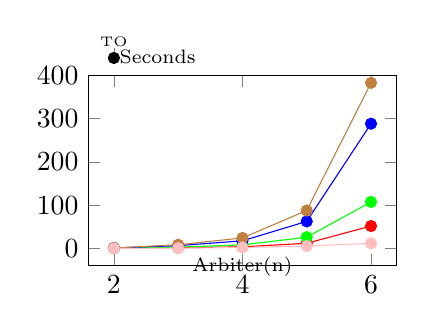
\begin{tikzpicture}
	\begin{axis}[name=Arbiter,height=4cm,width=5.5cm,
		xlabel=\scriptsize{Arbiter(n)},
		ylabel=\scriptsize{Seconds},
		x label style={at={(axis description cs:0.5,0.1)},anchor=north},
    	y label style={at={(axis description cs:0.07,1.1)},anchor=west,rotate=-90},
    	ymax=400,
		clip=false,
		legend pos=north west]
    % exp2
	\addplot[color=red,mark=*] coordinates {
		(2,1.3)
		(3,2.11)
		(4,4.3)
		(5,12.54)
		(6,52.34)
		%(6,37.703)
	};
	% exp4
	\addplot[color=green,mark=*] coordinates {
		(2,1.372)
		(3,3.545)
		(4,8.824)
		(5,26.531)
		(6,107.897)
	};
	% exp8
	\addplot[color=blue,mark=*] coordinates {
		(2,1.72)
		(3,7.022)
		(4,18.176)
		(5,63.028)
		(6, 288.419) 
	};
	%lineal10
	\addplot[color=brown,mark=*] coordinates {
		(2,1.737)
		(3,9.11)
		(4,24.866)
		(5,88.064)
		(6,382.565)
	};
	%Party
	\addplot[color=pink,mark=*] coordinates {
		(2,0.63)
		(3,1.18)
		(4,2.82)
		(5,6.12)
		(6,12.43)
	};
	%nocex
	\addplot[color=black,mark=*] coordinates {
	%	(1,0.511)
		(2,440)
	%	(3,14.807)
	%	(4,93.844)
	%	(5,600) %TO
	}node[pin={[pin distance=-0.1cm]90:{\tiny{TO}}}]{};

%\legend{exp2,exp4,exp8,lineal10,nocex}
    %\node[above right] at (rel axis cs:0, 1) {\;\;\scriptsize{T.O.:}};
	\end{axis}
\end{tikzpicture}
%Full Arbiter
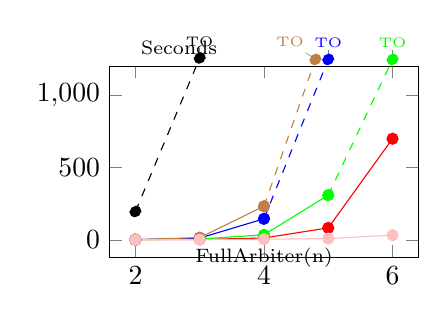
\begin{tikzpicture}
	\begin{axis}[name=FullArbiter,height=4cm,width=5.5cm,
		xlabel=\scriptsize{FullArbiter(n)},
		ylabel=\scriptsize{Seconds},
		x label style={at={(axis description cs:0.5,0.1)},anchor=north},
    	y label style={at={(axis description cs:0.07,1.1)},anchor=west,rotate=-90},
    	ymax=1200,
		clip=false,
		legend pos=north west]
    % exp2
	\addplot[color=red,mark=*] coordinates {
		(2,1.083)
		(3,2.774)
		(4,12.873)
		(5,82.981)
		(6,700.731)
		%(6,37.703)
	};
	% exp4
	\addplot[color=green,mark=*] coordinates {
		(2,1.24)
		(3,5.719)
		(4,34.7)
		(5,309.953)
	};
	\addplot[color=green,mark=*,dashed] coordinates {
		(5,309.953)
		(6,1250)
	}node[pin={[pin distance=-0.1cm]90:{\tiny{TO}}}]{};
	
	% exp8
	\addplot[color=blue,mark=*] coordinates {
		(2,1.55)
		(3,12.382)
		(4,145.86)
	};
	\addplot[color=blue,mark=*,dashed] coordinates {
		(4,145.86)
		(5,1250)
	}node[pin={[pin distance=-0.1cm]90:{\tiny{TO}}}]{};
	
	%lineal10
	\addplot[color=brown,mark=*] coordinates {
		(2,1.677)
		(3,15.45)
		(4,232.942)
		%(5,1250)%TO
	};
	\addplot[color=brown,mark=*,dashed] coordinates {
		(4,232.942)
		(4.8,1250)%TO
	}node[pin={[pin distance=-0.1cm]120:{\tiny{TO}}}]{};
	    
	%Party
	\addplot[color=pink,mark=*] coordinates {
		(2,0.68)
		(3,1.43)
		(4,4.078)
		(5,8.85)
		(6,32.73)
	};
	%nocex
	\addplot[color=black,mark=*,dashed] coordinates {
	%	(1,0.511)
		(2,196.115)
		(3,1260) % TO
	%	(4,93.844)
	%	(5,600) %TO
	}node[pin={[pin distance=-0.1cm]90:{\tiny{TO}}}]{};
	
%\legend{exp2,exp4,exp8,lineal10,nocex}
    %\node[above right] at (rel axis cs:0, 1) {\;\;\scriptsize{T.O.:}};
	\end{axis}
\end{tikzpicture}
%PNUELIARBITER
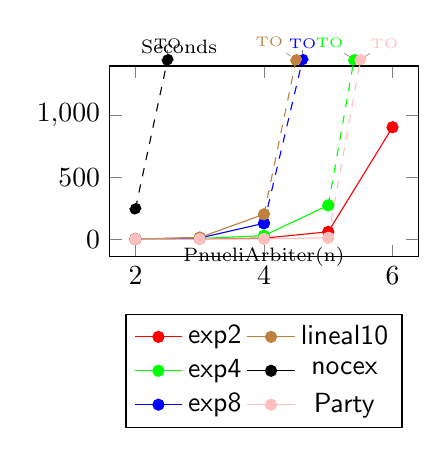
\begin{tikzpicture}
	\begin{axis}[name=PnueliArbiter,height=4cm,width=5.5cm,
		xlabel=\scriptsize{PnueliArbiter(n)},
		ylabel=\scriptsize{Seconds},
		x label style={at={(axis description cs:0.5,0.1)},anchor=north},
    	y label style={at={(axis description cs:0.07,1.1)},anchor=west,rotate=-90},
    	ymax=1400,
		clip=false,
		legend style={at={(0.5,-0.3)},anchor=north,legend  columns =3, transpose legend}]
    % exp2
     \addlegendimage{red, line legend, mark=*} % or mark=none?
    \addlegendentry{\textsf{exp2}}
    \addlegendimage{green, line legend, , mark=*} % or mark=none?
    \addlegendentry{\textsf{exp4}}
    \addlegendimage{blue, line legend, , mark=*} % or mark=none?
    \addlegendentry{\textsf{exp8}}
    \addlegendimage{brown, line legend, , mark=*} % or mark=none?
    \addlegendentry{\textsf{lineal10}}
    \addlegendimage{black,,line legend,  mark=*} % or mark=none?
    \addlegendentry{\textsf{nocex}}
    \addlegendimage{pink,line legend,  mark=*} % or mark=none?
    \addlegendentry{\textsf{Party}}
    % exp2
	\addplot[color=red,mark=*] coordinates {
		(2,1.206)
		(3,2.674)
		(4,8.639)
		(5,59.893)
		(6,905.203) % TO
		%(6,37.703)
	};
	% exp4
	\addplot[color=green,mark=*] coordinates {
		(2,1.406)
		(3,5.461)
		(4,29.063)
		(5,274.013)
	};
	\addplot[color=green,mark=*,dashed] coordinates {
		(5,274.013)
		(5.4,1450) 
	}node[pin={[pin distance=-0.1cm]110:{\tiny{TO}}}]{};
	
	% exp8
	\addplot[color=blue,mark=*] coordinates {
		(2,1.634)
		(3,9.749)
		(4,128.565)
	};
	\addplot[color=blue,mark=*,dashed] coordinates {
		(4,128.565)
		(4.6, 1450) %TO
	}node[pin={[pin distance=-0.1cm]90:{\tiny{TO}}}]{};
	%lineal10
	\addplot[color=brown,mark=*] coordinates {
		(2,1.789)
		(3,13.855)
		(4,201.653)
	};
	\addplot[color=brown,mark=*,dashed] coordinates {	
		(4,201.653)
		(4.5,1450)
	}node[pin={[pin distance=-0.1cm]130:{\tiny{TO}}}]{};
	%nocex
	\addplot[color=black,mark=*,dashed] coordinates {
	%	(1,0.511)
		(2,246.157)
	 	(2.5,1450)
	%	(4,93.844)
	%	(5,600) %TO
	}node[pin={[pin distance=-0.1cm]90:{\tiny{TO}}}]{};
	%party
	\addplot[color=pink,mark=*] coordinates {
		(2,0.69)
		(3,1.162)
		(4,2.408)
		(5,11.836)
		%(5.5,1450)
	};
	\addplot[color=pink,mark=*,dashed] coordinates {
		(5,11.836)
		(5.5,1450)
	}node[pin={[pin distance=-0.1cm]80:{\tiny{TO}}}]{};
    %\legend{exp2,exp4,exp8,lineal10,nocex,Party}
    %\node[above right] at (rel axis cs:0, 1) {\;\;\scriptsize{T.O.:}};
	\end{axis}
\end{tikzpicture}
\caption{Efficiency comparison for arbiter examples}\label{fig:arbiter-plots}
\end{wrapfigure}
To answer \textbf{RQ4} we have included in out analysis the synthesis tool {\PSketch}~\cite{Solar-Lezama+2008}, that implements a Counterexample-driven Guided Inductive Synthesis (CEGIS) algorithm to obtain code from sketched code (i.e., code annotated with ``holes''). To run {\PSketch}, we took the Dining Philosophers specification provided in~\cite{Solar-Lezama+2008}, and manually elaborated the specification for Mutex,  Readers-Writers, and the Barrier example.  The Peterson example cannot be analysed with  {\PSketch} since this tool only supports the analysis of safety properties.  For the arbiter case studies, we have compare against the tool {\Party} \cite{Party} which is a tool specifically tailored for distributed systems that use token ring architectures.

Our comparison focuses only on the time required by each technique for synthesizing the distributed solutions. The plots of Figs.~\ref{fig:examples-plot} and \ref{fig:arbiter-plots} depict the results of this comparison. In all the case studies, we notice that the efficiency of {\PSketch} is drastically affected as the number of processes to synthesize is incremented. For instance, in the dining philosophers with 6 processes, {\Sketch} timed out; in contrast, our tool was able to obtain a solution. Similarly, in the case of 1 reader and 6 writers, {\PSketch} failed in synthesizing a solution, while our approach succeeded. A similar analysis applies to Mutex.

  In the case of the tool {\Party}, for the \textsf{arb} and \textsf{farb} examples {\Party} was able to find solutions faster than \textsf{exp2}; it must be noted that in these cases {\Party} uses a cut-off of $4$,  i.e., it reduces configurations with $n>4$ processes to the case $n=4$.  However,  even though {\Party} has several optimizations for token ring systems, our tool was able to synthesize an implementation of the \textsf{parb(6)} and {\Party} timed out for this case. 
  
It is worth noting that the tool can be used to find different solutions for some examples.  We have experimented with this using the \textsf{phil} example, where, after finding an initial solution, we allow the algorithm to keep looking for further solutions, and it succeeded in finding a second solution.  For space reasons we do not investigate this aspect of the tool further here.

%For instance, for the dining philosophers, the first found solution is one in which each philosopher takes a fork only if her two forks are available (a know solution to prevent deadlock). When we allow the algorithm to keep looking for further solutions, it succeeded in finding a second solution, the ``even/odd'' solution, where $n-1$ philosophers take first their left fork and after their right fork, whereas  philosopher $n$ takes first her right fork and then her left fork.  
